\documentclass{article}
\usepackage[utf8]{inputenc} %кодировка
\usepackage[T2A]{fontenc}
\usepackage[english,russian]{babel} %русификатор 
\usepackage{mathtools} %библиотека матеши
\usepackage[left=1cm,right=1cm,top=2cm,bottom=2cm,bindingoffset=0cm]{geometry} %изменение отступов на листе
\usepackage{amsmath}
\usepackage{graphicx} %библиотека для графики и картинок
\graphicspath{}
\DeclareGraphicsExtensions{.pdf,.png,.jpg}
\usepackage{subcaption}
\usepackage{pgfplots}
\usepackage{float}
\usepackage{listings}
\usepackage{hyperref}
\usepackage{physics}
\usepackage{xcolor}

\lstset{language=Java,
        basicstyle=\ttfamily,
        keywordstyle=\color{blue}\ttfamily,
        stringstyle=\color{red}\ttfamily,
        commentstyle=\color{green}\ttfamily,
        morecomment=[l][\color{magenta}]{\#},
        captionpos=b,
        frame=single % рамка вокруг кода
}

\begin{document}
% НАЧАЛО ТИТУЛЬНОГО ЛИСТА
\begin{center}
    \Large
    Федеральное государственное автономное \\
    образовательное учреждение высшего образования \\ 
    «Научно-образовательная корпорация ИТМО»\\
    \vspace{0.5cm}
    \large
    Факультет программной инженерии и компьютерной техники \\
    Направление подготовки 09.03.04 Программная инженерия \\
    \vspace{1cm}
    \Large
    \textbf{Отчёт по лабораторной работе №5} \\
    По дисциплине «Вычислительная математика» (4 семестр)\\
    \large
    \vspace{8cm}

    \begin{minipage}{.33\textwidth}
    \end{minipage}
    \hfill
    \begin{minipage}{.4\textwidth}
    
        \textbf{Студент}: \vspace{.1cm} \\
        \ Дениченко Александр P3212\\
        \textbf{Практик}:  \\
        \ Наумова Надежда Александровна
    \end{minipage}
    \vfill
Санкт-Петербург\\ 2024 г.
\end{center}
\pagestyle{empty}
% КОНЕЦ ТИТУЛЬНОГО ЛИСТА 
\newpage
\pagestyle{plain}
\section{Цель работы}
Решить задачу интерполяции, найти значения функции при заданных значениях аргумента, отличных от узловых точек.
\section{Вычислительная часть}
1. Выбрать из табл. 1 заданную по варианту таблицу y = f(x) (таблица 1.1 – таблица 1.5);\\
2. Построить таблицу конечных разностей для заданной таблицы. Таблицу отразить в отчете;\\
3. Вычислить значения функции для аргумента $X_1$ (см. табл.1), используя первую или вторую интерполяционную формулу Ньютона. Обратить внимание какой конкретно формулой необходимо воспользоваться;\\
4. Вычислить значения функции для аргумента $X_2$ (см. табл. 1), используя первую или вторую интерполяционную формулу Гаусса. Обратить внимание какой конкретно формулой необходимо воспользоваться;\\
5. Подробные вычисления привести в отчете.\\ \\
\textbf{Трассировка по варианту:}
\begin{table}[H]
    \centering
    \caption{Трассировка}
    \begin{tabular}{|c|c|c|c|c|}
    \hline
    x & y & № варианта & \( X_1 \) & \( X_2 \) \\ \hline
    1,10 & 0,2234 &  & 1,121 & 1,482 \\ \hline
    1,25 & 1,2438 & 8 & 1,852 & 1,652 \\ \hline
    1,40 & 2,2644 &  & 1,168 & 1,463 \\ \hline
    1,55 & 3,2984 &  & 1,875 & 1,575 \\ \hline
    1,70 & 4,3222 &  & 1,189 & 1,491 \\ \hline
    1,85 & 5,3516 &  & 1,891 & 1,671 \\ \hline
    2,00 & 6,3867 &  & 1,217 & 1,473 \\ \hline
    \end{tabular}
\end{table}
    
\section{Решение}

\begin{table}[H]
    \centering
    \caption{Конечные разности}
    \begin{tabular}{|c|c|c|c|c|c|c|c|c|}
    \hline
        Gauss&$x_i$ & $y_i$ & $\Delta y_i$ & $\Delta^2 y_i$ & $\Delta^3 y_i$ & $\Delta^4 y_i$ & $\Delta^5 y_i$ & $\Delta^6 y_i$ \\ \hline
        -3&1,10& 0,2234 & 1,0204 & 0,0002 & 0,0132 & -0,0368 & 0,0762 & -0,1313 \\ \hline
        -2&1,25& 1,2438 & 1,0206 & 0,0134 & -0,0236 & 0,0394 & -0,0551 \\ \hline
        -1&1,40& 2,2644 & 1,0340 & -0,0102 & 0,0158 & -0,0157 \\ \hline
        0&1,55& 3,2984 & 1,0238 & 0,0056 & 0,0001 \\ \hline
        1&1,70& 4,3222 & 1,0294 & 0,0057 \\ \hline
        2&1,85& 5,3516 & 1,0351\\ \hline
        3&2,00& 6,3867 \\ \hline
    \end{tabular}
\end{table}
\textbf{Метод Ньютона}\\
\[h_x = 0.15\]
\[t = \frac{x-x_0}{0.15}\]
Для $x_1 = 1.852$:
\[t = \frac{1.852-2.00}{0.15} = -0.987\]
Так как $x_1$ лежит ближе к концу набора данных, то будем исопльзовать вторую формулу Ньютона:
\[N_6(x) = 6.3867 
+ (-0.987)\cdot 1.0351 
+ \frac{(-0.987)(-0.987+1)}{2!}\cdot 0.0057 +\]

\[+ \frac{(-0.987)(-0.987+1)(-0.987+2)}{3!}\cdot 0.0001
+ \frac{(-0.987)(-0.987+1)(-0.987+2)(-0.987+3)}{4!}\cdot (-0.0157) +\]

\[+ \frac{(-0.987)(-0.987+1)(-0.987+2)(-0.987+3)(-0.987+4)}{5!}\cdot (-0.0551) +\]
\[+ \frac{(-0.987)(-0.987+1)(-0.987+2)(-0.987+3)(-0.987+4)(-0.987+5)}{6!}\cdot (-0.1313)  =  
5.3651 \]
Для $x_2 = 1.652$:
\[t = \frac{1.652-1.10}{0.15} = 3.68\]
Так как $x_2$ лежит ближе к концу набора данных, то будем исопльзовать вторую формулу Ньютона:
\[N_6(x) =
    0.2234+3.68\cdot 1.0204+ \frac{3.68(3.68-1)}{2!}\cdot0.0002 +
\]
\[+
    \frac{3.68(3.68-1)(3.68-2)}{3!}\cdot0.0132 + \frac{3.68(3.68-1)(3.68-2)(3.68-3)}{4!}\cdot(-0.0368) +
\]
\[+
    \frac{3.68(3.68-1)(3.68-2)(3.68-3)(3.68-4)}{5!}\cdot0.0762 +
    \frac{3.68(3.68-1)(3.68-2)(3.68-3)(3.68-4)(3.68-5)}{6!}\cdot(-0.1313) = 
    3.9955
\]\\
\textbf{Метод Гаусса}\\
\[a = 1.55\]
\[x = 1.852\]
\[1.852 > a\]
\[t = \frac{1.852 - 1.55}{0.15} = 2.013\]
\[
    P_6(x) = 3.2984 + (2.013 \cdot 1.0238) + \frac{2.013(2.013-1)}{2} \cdot 0.0056 + \frac{2.013(2.013-1)(2.013-2)}{6} \cdot 0.0001 + 
\]
\[+
\frac{2.013(2.013-1)(2.013-2)(2.013-3)}{24} \cdot (-0.0368) + \frac{2.013(2.013-1)(2.013-2)(2.013-3)(2.013-4)}{120} \cdot 0.0762 = 5.3651
\]


\[x = 1.652\]
\[1.652 > a\]
\[t = \frac{1.652 - 1.55}{0.15} = 0.68\]

\[
    P_6(x) = 3.2984 + (0.68 \cdot 1.0238) + \frac{0.68(0.68-1)}{2} \cdot 0.0056 + \frac{0.68(0.68-1)(0.68-2)}{6} \cdot 0.0001 + 
\]
\[+
\frac{0.68(0.68-1)(0.68-2)(0.68-3)}{24} \cdot (-0.0368) + \frac{0.68(0.68-1)(0.68-2)(0.68-3)(0.68-4)}{120} \cdot 0.0762 = 3.994 +0.0024 = 3.996
\]
\section{Программная часть}

1. Исходные данные задаются тремя способами:\\

a) в виде набора данных (таблицы x,y), пользователь вводит значения с клавиатуры;

b) в виде сформированных в файле данных (подготовить не менее трех тестовых
вариантов);

c) на основе выбранной функции, из тех, которые предлагает программа, например, sin(x). Пользователь выбирает уравнение, исследуемый интервал и количество точек на интервале (не менее двух функций).\\ \\
2. Сформировать и вывести таблицу конечных разностей;\\
3. Вычислить приближенное значение функции для заданного значения аргумента, введенного с клавиатуры, указанными методами (см. табл. 2). Сравнить полученные значения;\\
4. Построить графики заданной функции с отмеченными узлами интерполяции и интерполяционного многочлена Ньютона/Гаусса (разными цветами);\\
5. Программа должна быть протестирована на различных наборах данных, в том числе и некорректных.\\
6. Проанализировать результаты работы программы.
\\ \\
\textbf{Необязательное задание (до 20 баллов):}

1. Реализовать в программе вычисление значения функции для заданного значе-
ния аргумента, введенного с клавиатуры, используя схемы Стирлинга;

2. Реализовать в программе вычисление значения функции для заданного значе-
ния аргумента, введенного с клавиатуры, используя схемы Бесселя.

\section{Машинная реализация}
\begin{lstlisting}[caption={Реализация метода Лагранжа для интерполяции значений.}]
@Override
public void calculate() {
    double v = this.arg;
    double sum = 0.0;

    for (int i = 0; i < this.size; i++) {
        double term = 1.0;
        for (int j = 0; j < this.size; j++) {
            if (j != i) {
                term *= (v - this.xVal.get(j)) / (this.xVal.get(i) - this.xVal.get(j));
            }
        }
        sum += this.yVal.get(i) * term;
    }
    logger.info(sum + "");
    this.interpolatedValue = sum;
}
\end{lstlisting}

\begin{lstlisting}[caption={Реализация метода Ньютона для интерполяции значений.}]
public void calculate() {
    initializeDividedDifferenceTable();
    computeDividedDifferences();

    double v = this.arg;
    double sum = this.yVal.get(0);
    for (int i = 1; i < this.size; i++) {
        double term = 1.0;
        for (int j = 0; j < i; j++) {
            term *= (v - this.xVal.get(j));
        }
        sum += term * this.dividedDifferences.get(0).get(i);
    }
    this.interpolatedValue = sum;
}

private void initializeDividedDifferenceTable() {
    for (int i = 0; i < this.size; i++) {
        dividedDifferences.add(new ArrayList<>());
        dividedDifferences.get(i).add(this.yVal.get(i));
    }
}

private void computeDividedDifferences() {
    for (int i = 1; i < this.size; i++) {
        for (int j = 0; j < this.size - i; j++) {
            double diff = dividedDifferences.get(j + 1).get(i - 1) -
            - dividedDifferences.get(j).get(i - 1);
            double denom = this.xVal.get(j + i) - this.xVal.get(j);
            double dividedDifference = diff / denom;
            dividedDifferences.get(j).add(dividedDifference);
        }
    }
}
\end{lstlisting}

\begin{lstlisting}[caption={Реализация метода Гаусса для интерполяции значений.}]
public void calculate() {
    double[] y_diff = new double[size];
    for (int i = 0; i < size; i++) {
        y_diff[i] = yVal.get(i);
    }

    double x_target = arg;
    double h = xVal.get(1) - xVal.get(0);
    int n = (size - 1) / 2;
    int nearestIndex = findNearestIndex(x_target);

    double p = (x_target - xVal.get(nearestIndex)) / h;
    interpolatedValue = y_diff[nearestIndex];

    if (nearestIndex <= n) {
        logger.info("Forward interpolation");
        for (int i = 1; i <= n; i++) {
            for (int j = nearestIndex; j < size - i; j++) {
                y_diff[j] = y_diff[j + 1] - y_diff[j];
            }
            double term = p;
            for (int k = 1; k < i; k++) {
                term *= (p - k) / (k + 1);
            }
            interpolatedValue += term * y_diff[nearestIndex];
        }
    } else {
        logger.info("Backward interpolation");
        for (int i = 1; i <= n; i++) {
            for (int j = nearestIndex; j >= i; j--) {
                y_diff[j] = y_diff[j] - y_diff[j - 1];
            }
            double term = p;
            for (int k = 1; k < i; k++) {
                term *= (p + k) / (k + 1);
            }
            interpolatedValue += term * y_diff[nearestIndex - i + 1];
        }
    }
    nodesForGraph();
}
\end{lstlisting}

\begin{lstlisting}[caption={Реализация метода Бесселя для интерполяции значений.}]
public void calculate() {
    int n = xVal.size();
    double tSub = (arg - xVal.get(n / 2)) / (xVal.get(1) - xVal.get(0));
    if ((size % 2 != 0) || (Math.abs(tSub) > 0.75) || (Math.abs(tSub) < 0.25)) {
        logger.info(String.valueOf(tSub));
        return;
    }
    for (int i = 0; i < n; i++) {
        defy.get(i).set(0, yVal.get(i));
    }

    for (int i = 1; i < n; i++) {
        for (int j = 0; j < n - i; j++) {
            defy.get(j).set(i, defy.get(j + 1).get(i - 1) - defy.get(j).get(i - 1));
        }
    }
    n = xVal.size() - 1;
    int center = n / 2;
    double a = xVal.get(center);
    double t = (arg - a) / (xVal.get(1) - xVal.get(0));
    double result = (defy.get(center).get(0) + defy.get(center + 1).get(0))
     * 0.5 + (t - 0.5) * defy.get(center).get(1) + t * (t - 1)
      * 0.5 * (defy.get(center - 1).get(2) + defy.get(center).get(2)) * 0.5;
    double term = t * (t - 1) / 2;
    for (int k = 3; k < n + 1; k++) {
        if (k % 2 == 0) {
            term /= (t - 0.5);
            term *= (t + (k * 0.5 - 1)) * (t - (k * 0.5)) / k;
            result += term * (defy.get((int) (center - 1 - (k * 0.5 - 1))).get(k) 
            + defy.get((int) (center - (k * 0.5 - 1))).get(k)) / 2;
        } else {
            term *= (t - 0.5) / k;
            result += term * defy.get(center - k / 2).get(k);
        }
    }
    interpolatedValue = result;
}
\end{lstlisting}

\begin{lstlisting}[caption={Реализация метода Стирлинга для интерполяции значений.}]
public void calculate() {
    int n = xVal.size();
    double tSub = (arg - xVal.get(n / 2)) / (xVal.get(1) - xVal.get(0));
    logger.info(String.valueOf(tSub));
    if ((size % 2 == 0) || (Math.abs(tSub) > 0.25)) {
        return;
    }

    for (int i = 0; i < n; i++) {
        defy.get(i).set(0, yVal.get(i));
    }

    for (int i = 1; i < n; i++) {
        for (int j = 0; j < n - i; j++) {
            defy.get(j).set(i, defy.get(j + 1).get(i - 1) - defy.get(j).get(i - 1));
        }
    }

    n = xVal.size() - 1;
    int center = n / 2;
    double a = xVal.get(center);
    double t = (arg - a) / (xVal.get(1) - xVal.get(0));

    double result = defy.get(center).get(0) + t * (defy.get(center - 1).get(1) 
    + defy.get(center).get(1))*0.5 + (Math.pow(t, 2))* 0.5 * defy.get(center - 1).get(2);
    double term = (Math.pow(t, 2))* 0.5;

    for(int k = 3; k < n; k++) {
        if(k % 2 == 0){
            term *= t / k;
            result =result + term * defy.get((center - k/2)).get(k);
        }
            else{
            term *= (Math.pow(t, 2) - (int)Math.pow(k*0.5, 2))/ (k * t);
            result += term * (defy.get((center - k/2 - 1)).get(k) 
            + defy.get((center - k/2)).get(k))*0.5;
        }

    }
    interpolatedValue = result;
}
\end{lstlisting}

\section{Схемы}
\begin{center}
    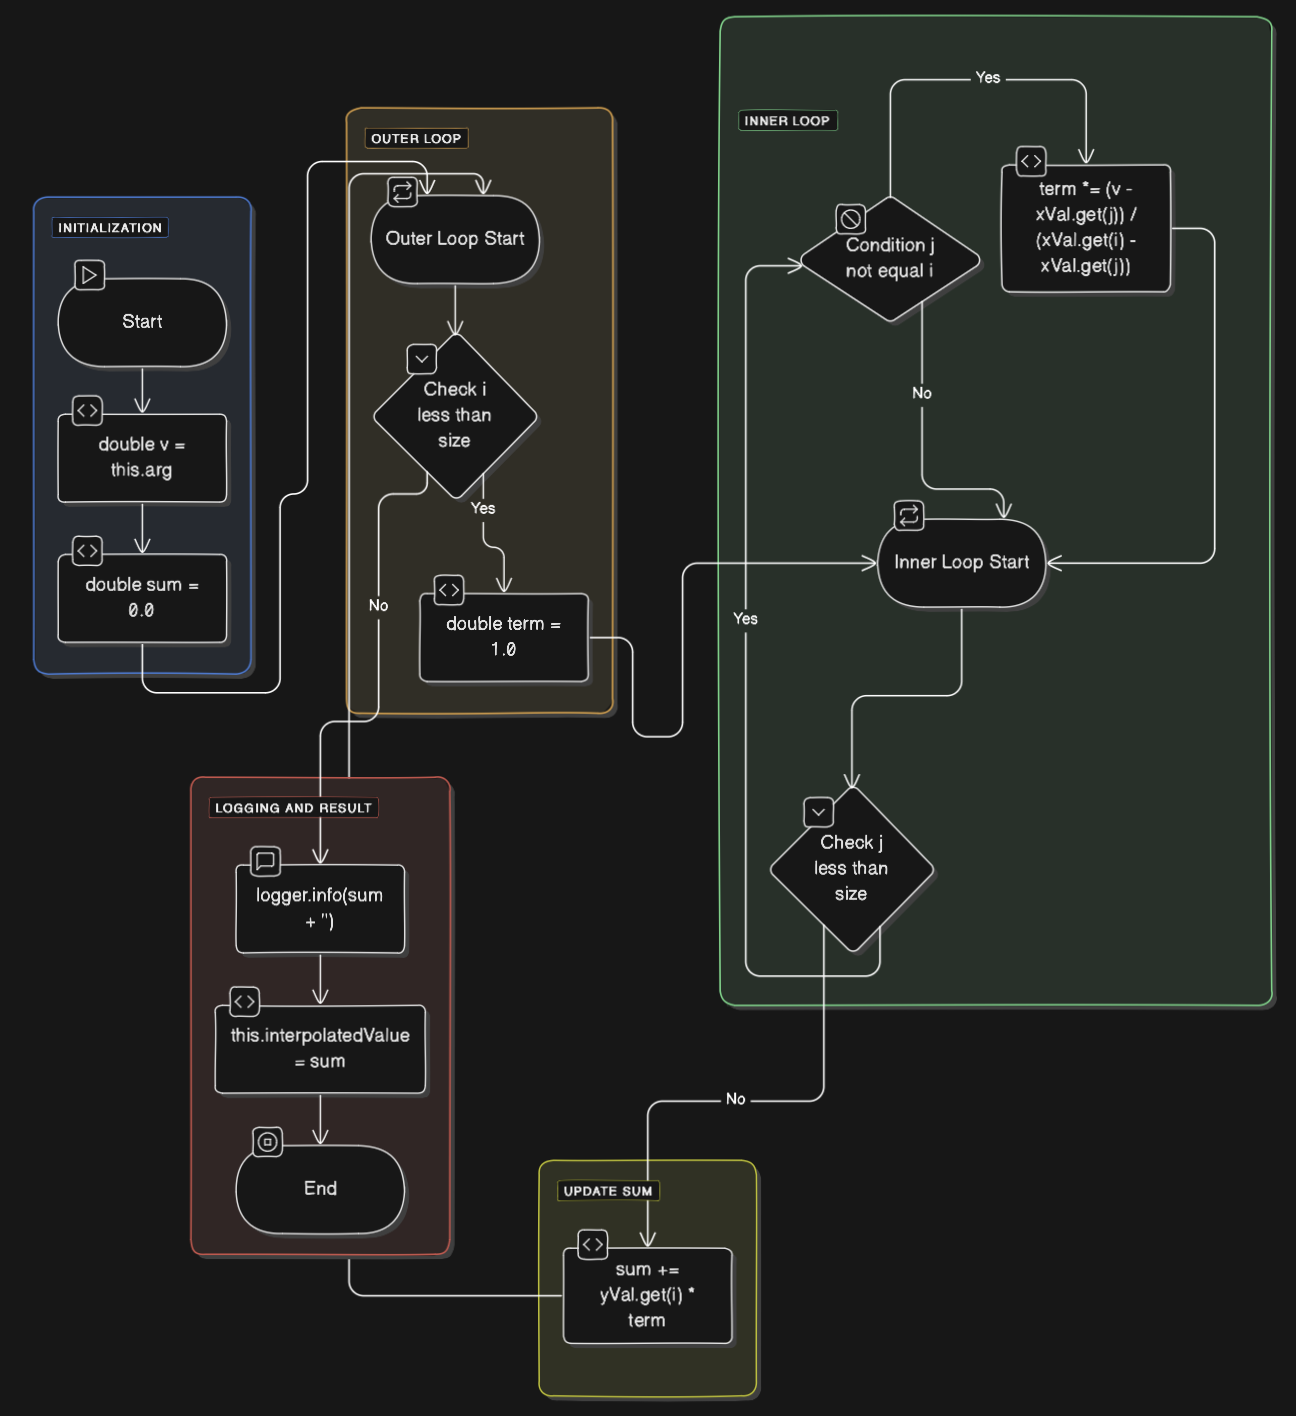
\includegraphics[width=.7\textwidth]{lagr.png}\\
    \textbf{Схема 1: Лагранж}
\end{center}
\begin{center}
    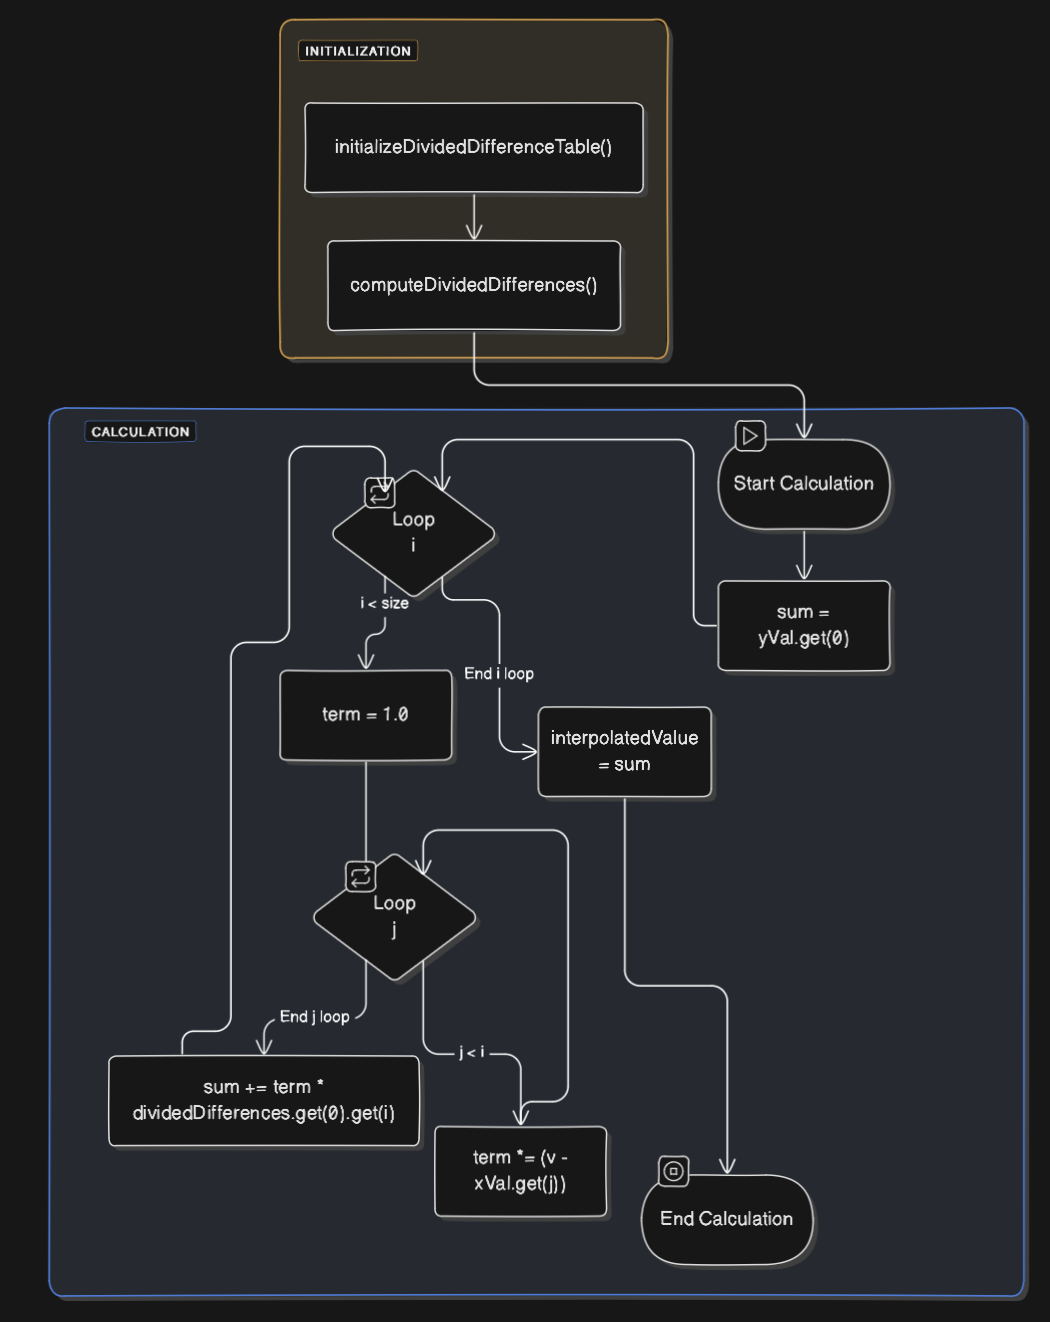
\includegraphics[width=.9\textwidth]{newt.png}\\
    \textbf{Схема 2: Ньютон}
\end{center}
\begin{center}
    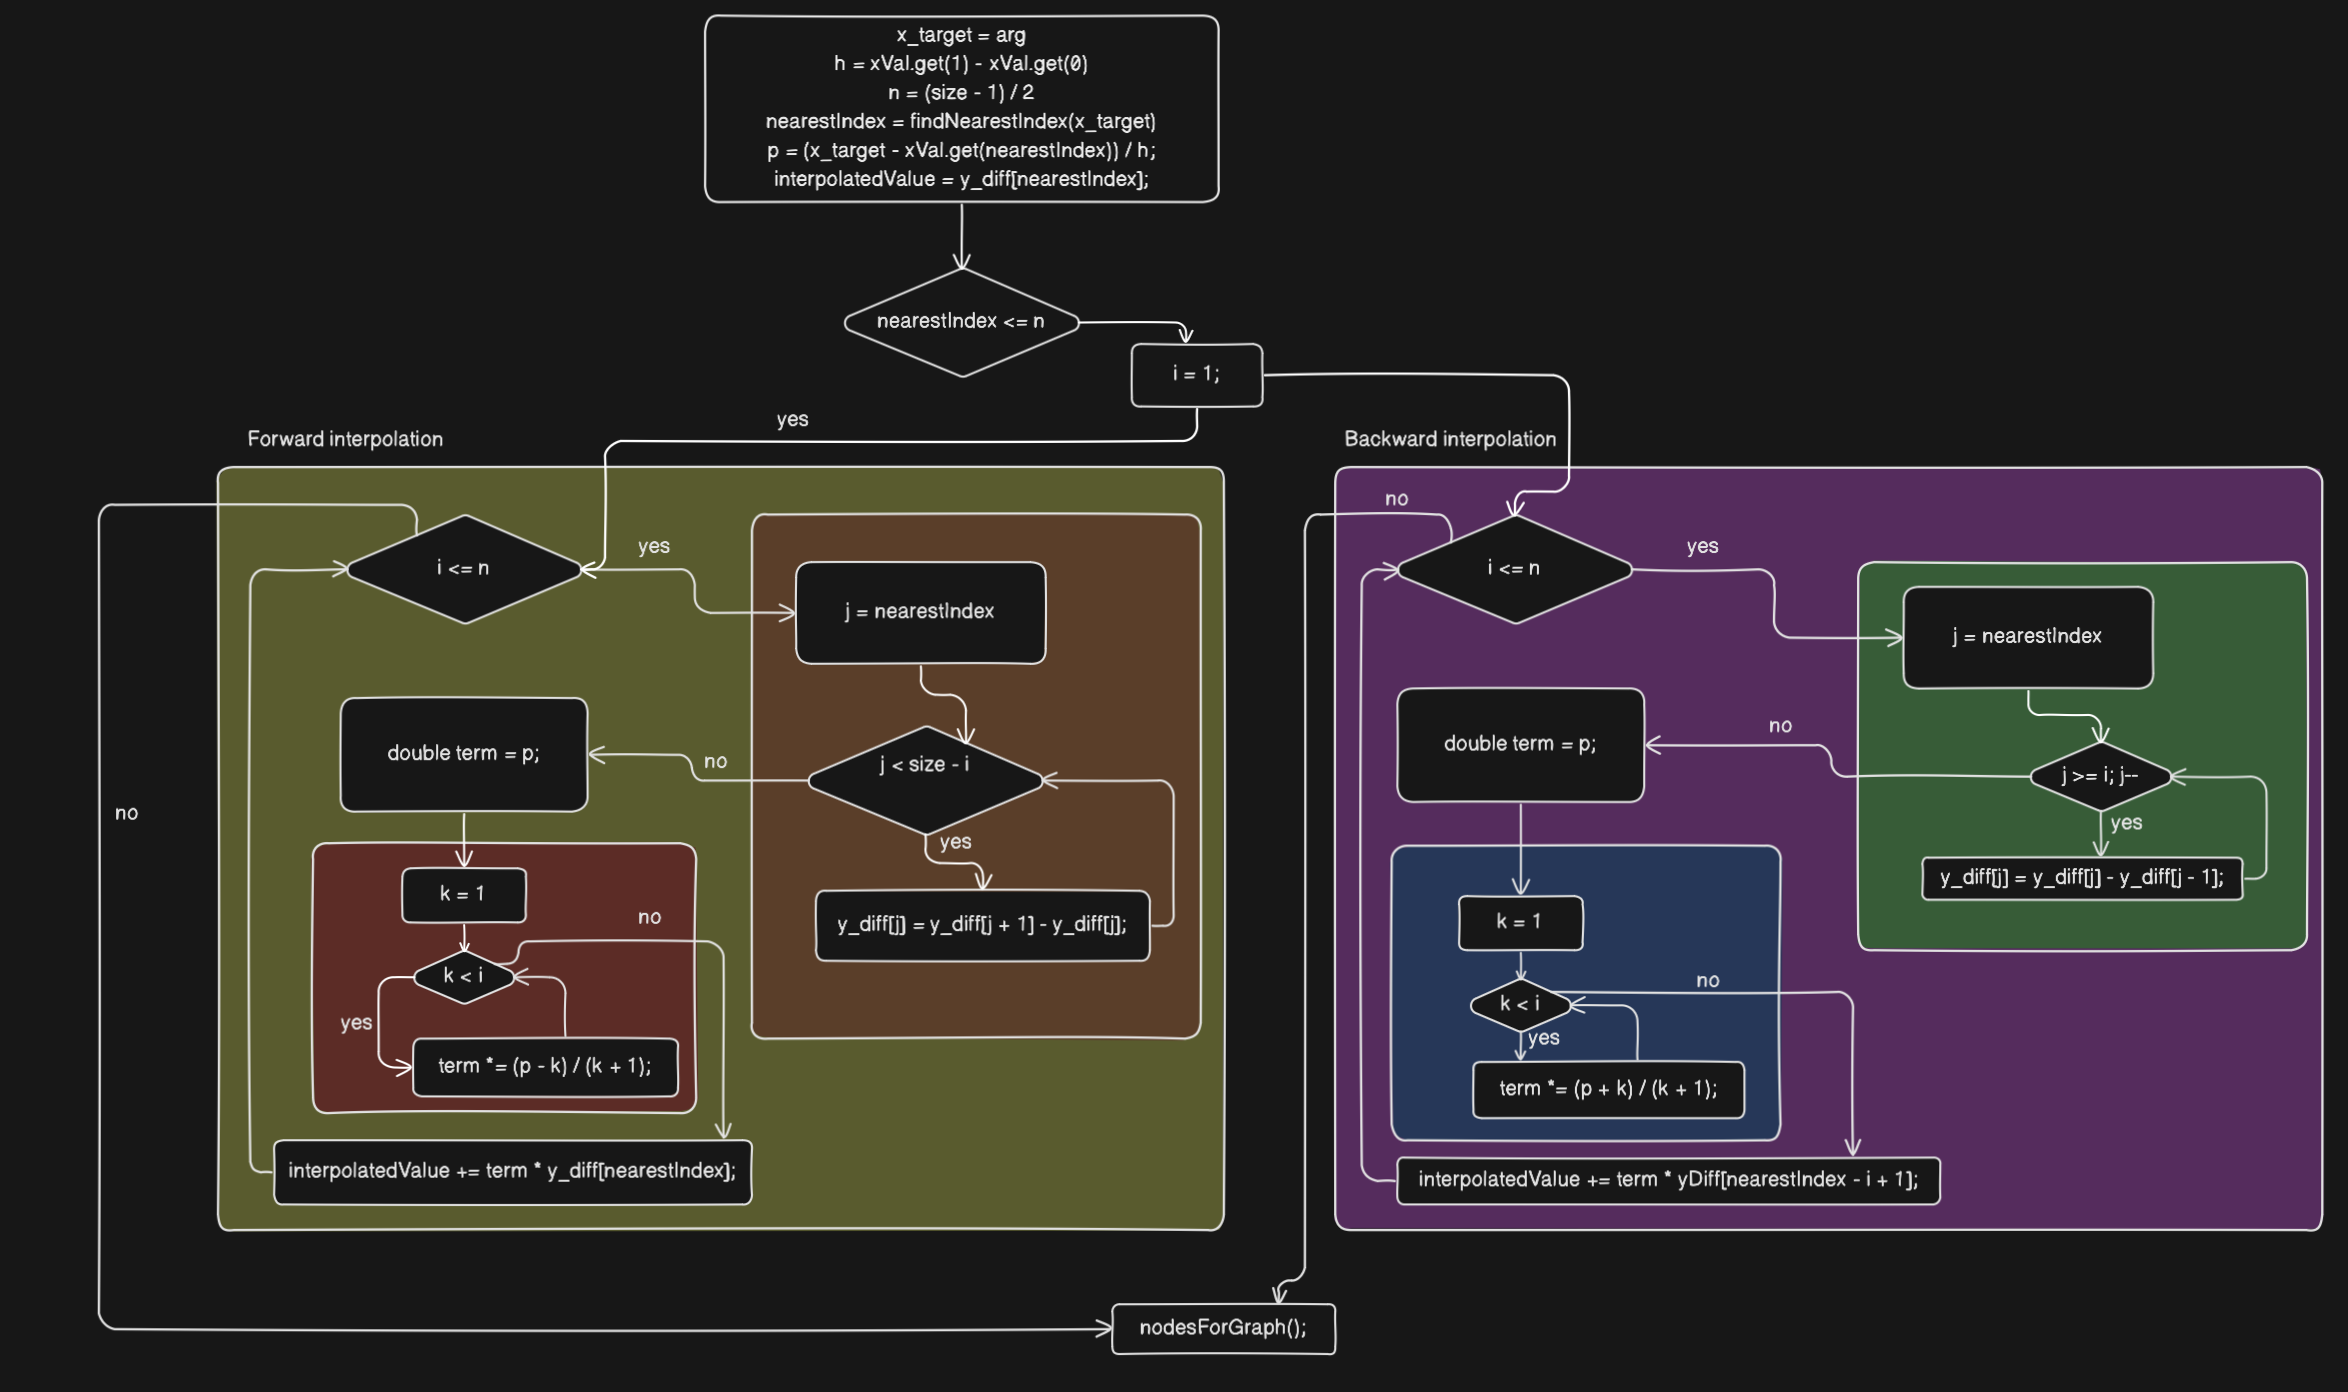
\includegraphics[width=.9\textwidth]{gauss.png}\\
    \textbf{Схема 3: Гаусс}
\end{center}
\begin{center}
    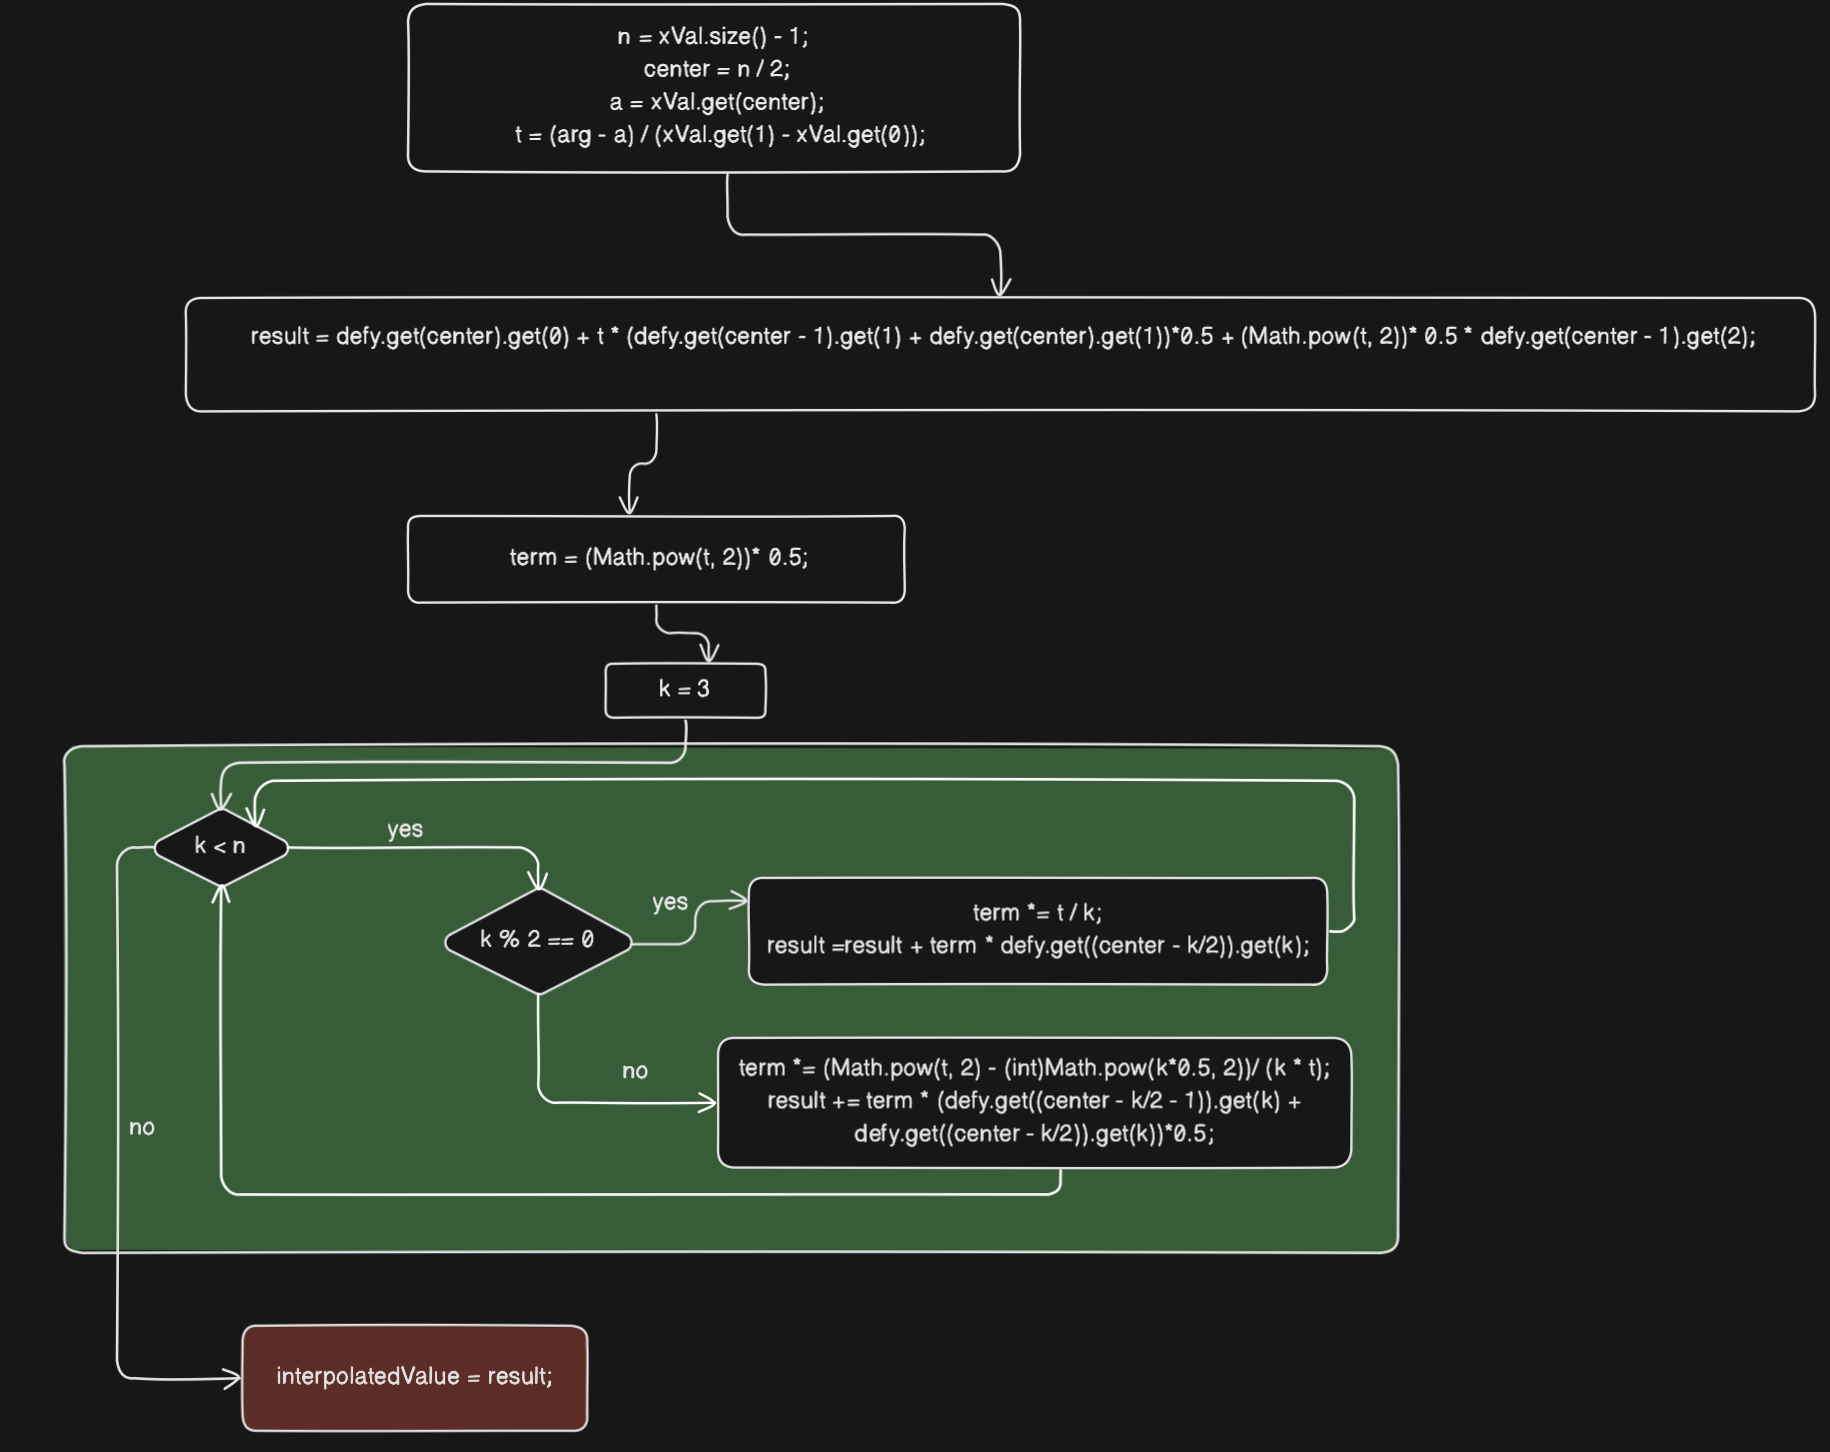
\includegraphics[width=.9\textwidth]{stirl.png}\\
    \textbf{Схема 4: Стирлинг}
\end{center}
\begin{center}
    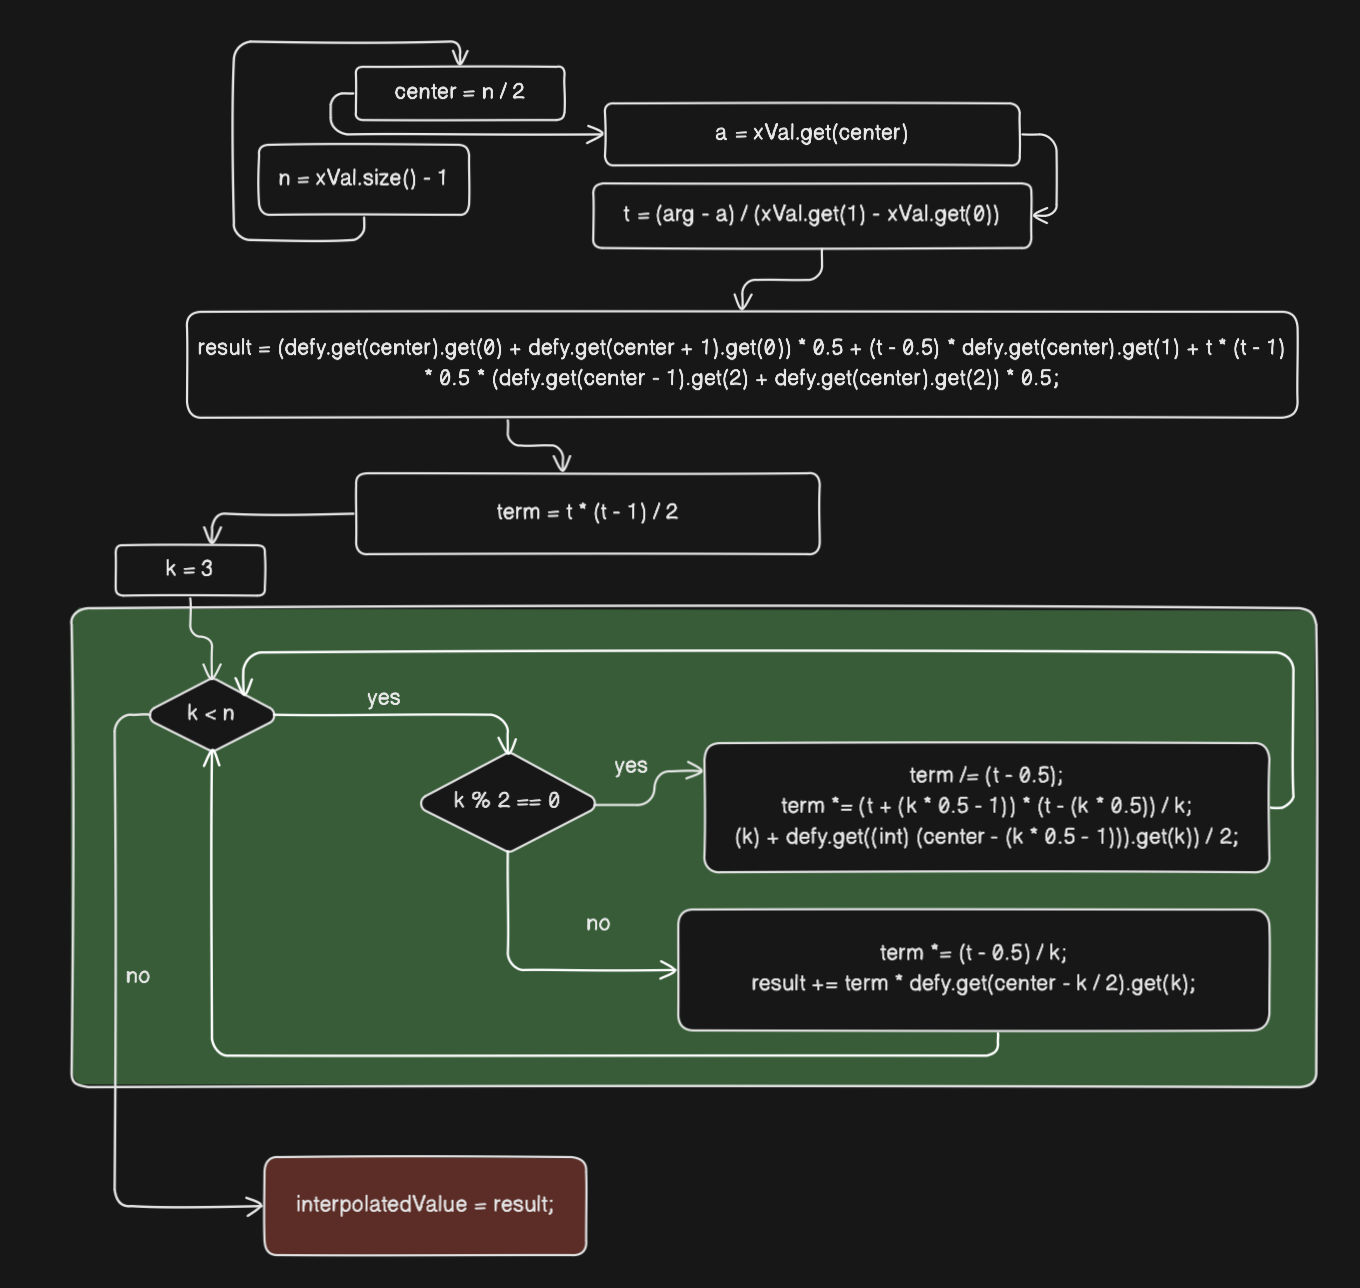
\includegraphics[width=.9\textwidth]{bessel.png}\\
    \textbf{Схема 5: Бессель}
\end{center}

\section{GitHub}
Ссылка на мой репозиторий на GitHub: \url{https://github.com/Alex-de-bug/cm_math/tree/main/lab5}.

\section{Вывод}
При выполнении работы были изучены методы интерполяции, очень много проблем создали механизмы Java, но тем не менее разработано веб приложение и проведено тестирование на разных наборах данных. Методы дают примерно одинаковые значения, погреность невилируемая.
\end{document}
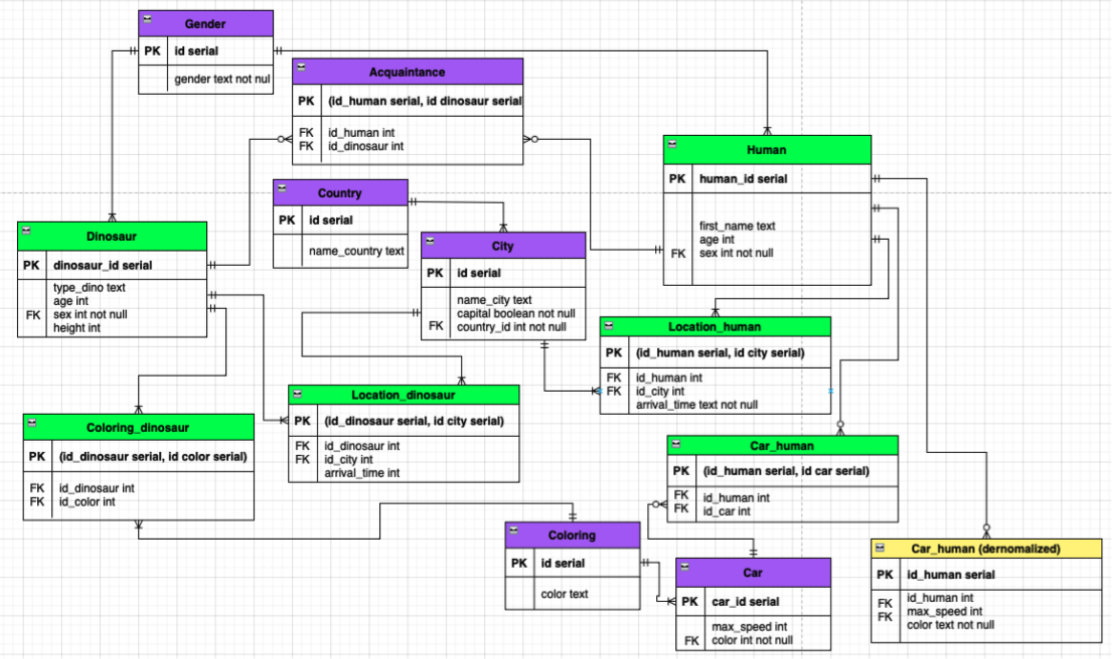
\includegraphics[width=.9\textwidth]{123}